\documentclass[12pt,letterpaper]{article}
\usepackage[utf8]{inputenc}
\usepackage[spanish]{babel}
\usepackage{amsmath}
\usepackage{amsfonts}
\usepackage{amssymb}
\usepackage{makeidx}
\usepackage{natbib}
\usepackage{graphicx}
\usepackage{lmodern}
\usepackage{kpfonts}
\usepackage{fourier}
\usepackage{pdfpages}
\usepackage[left=4cm,right=4cm,top=3cm,bottom=3cm]{geometry}

\author{Everardo Estrella Rojo}

\title{Tarea EV 1 3 Investigaci\'on de par de rotaci�n y cuaternios}

\date{Martes 17 de Septiembre 2019}

\begin{document}   %cabeza

\maketitle
\section{Par de Rotaci\'on}
El par motor es el momento de fuerza que ejerce un motor sobre el eje de transmisi�n de potencia o, dicho de otro modo, la tendencia de una fuerza para girar un objeto alrededor de un eje, punto de apoyo, o de pivote. La potencia desarrollada por el par motor es proporcional a la velocidad angular del eje de transmisi�n, viniendo dada por:

\begin{equation}
P=Mw
\end{equation}
Mediante la definici�n de un vector k (kx,ky.kz) y un �ngulo de giro ? , tal que el sistema OUVW corresponde al sistema OXYZ girado un �ngulo ? sobre el eje k

\begin{figure}[h!] 
\centering
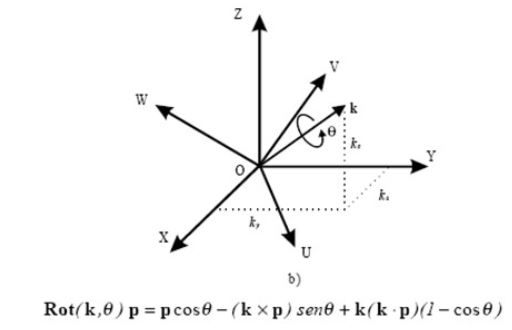
\includegraphics[scale=0.5]{Par1.jpg}
\caption{Par de Rotaci\'on}
\end{figure}

\section{Cuaternios}

\newpage
\includepdf[pages=-]{Tarea 1}

\section{Conclusion}
me agrado el tema \citep{adams1995hitchhiker}

\bibliographystyle{plain}
\bibliography{references}
\end{document}
